\documentclass[10pt, compress]{beamer}
\usetheme{m}
\usepackage{booktabs}
\usepackage[ampersand]{easylist}
\usepackage{minted}
\usemintedstyle{manni}
\usepgfplotslibrary{dateplot}

\title{Satellid: Personal Knowledge Manager}
\subtitle{with Web Technologies}
\date{18 March 2015}
\author{Muhammad Haidar Hanif}
\institute{Gunadarma University}

\begin{document}

% ============================================================

\maketitle

% ============================================================

\begin{frame}[fragile]
  \frametitle{Outline}

  \begin{description}
    \item[Introduction]: Background, Problem Statements, Objectives, Scope
    \item[Literature Study]: KMS, SDLC, Design Pattern, Database, Programming, Platform, Framework, Soft. Testing, SCM
    \item[Analysis \& Design]: Target User, User Types, User Stories, Contextual System, Functionality Flow, App Architecture, User Interface \& Interaction
    \item[Implementation \& Testing]: Agile Development, Code, and Test
    \item[Conclusion \& Suggestion]
  \end{description}

\end{frame}

% ============================================================

\section{Introduction}

% ------------------------------------------------------------

\begin{frame}[fragile]

  \begin{center}
  There are tons of daily personal knowledge that must be managed, but can't be handled with regular tools.
  \end{center}

\end{frame}

% ------------------------------------------------------------

\begin{frame}[fragile]

  \begin{center}
  How to manage tons of daily personal knowledge we have with just a simple and single system of knowledge manager that implemented with Web technologies?
  \end{center}

\end{frame}

% ------------------------------------------------------------

\begin{frame}[fragile]
  \frametitle{Introduction: Background}

  \begin{block}{Background}
    Solve a problem around \alert{\emph{daily knowledge management}}.\\
    Need for tool and system to make it more effective.
    ...
  \end{block}

\end{frame}

% ------------------------------------------------------------

\begin{frame}[fragile]
  \frametitle{Introduction: Problem Definition}

  \begin{block}{Problem Definition}
    \begin{enumerate}
      \item How to manage tons of personal or even collective knowledge we have with just a simple and single system of knowledge manager?
      \item How can knowledge manager naturally structure the data into knowledge that has context?
    \end{enumerate}
  \end{block}

\end{frame}

% ------------------------------------------------------------

\begin{frame}[fragile]
  \frametitle{Introduction: Objectives}

  \begin{block}{Objectives}
    \begin{itemize} \itemsep0pt
      \item Define and develop a new kind of knowledge management system (KMS) or knowledge manager called \alert{``Satellid knowledge manager''} to met the solution.
      \item It utilize knowledge template which use context and structure, to store and managing personal daily knowledge.
      \item Developed and built using Web technologies.
    \end{itemize}
  \end{block}

\end{frame}

% ------------------------------------------------------------

\begin{frame}[fragile]
  \frametitle{Introduction: Problem Scope}

  \begin{block}{Scope}
    \begin{itemize} \itemsep0pt
      \item \alert{Create a \emph{simpler system}} to do daily knowledge management for personal use with \alert{basic \textsc{browse, read, edit, add, delete} (BREAD) features}.
      \item The main methodologies are agile, MVP, and ATDD.
      \item The tools are MongoDB, JavaScript/CoffeeScript, JSON, Node.js, Meteor framework, and Git.
    \end{itemize}
  \end{block}

\end{frame}

% ============================================================

\section{Literature Study}

% ------------------------------------------------------------

\begin{frame}
  \frametitle{Literature Study}

  \begin{figure}[ht]
    \vspace{-25pt}
    \centering
    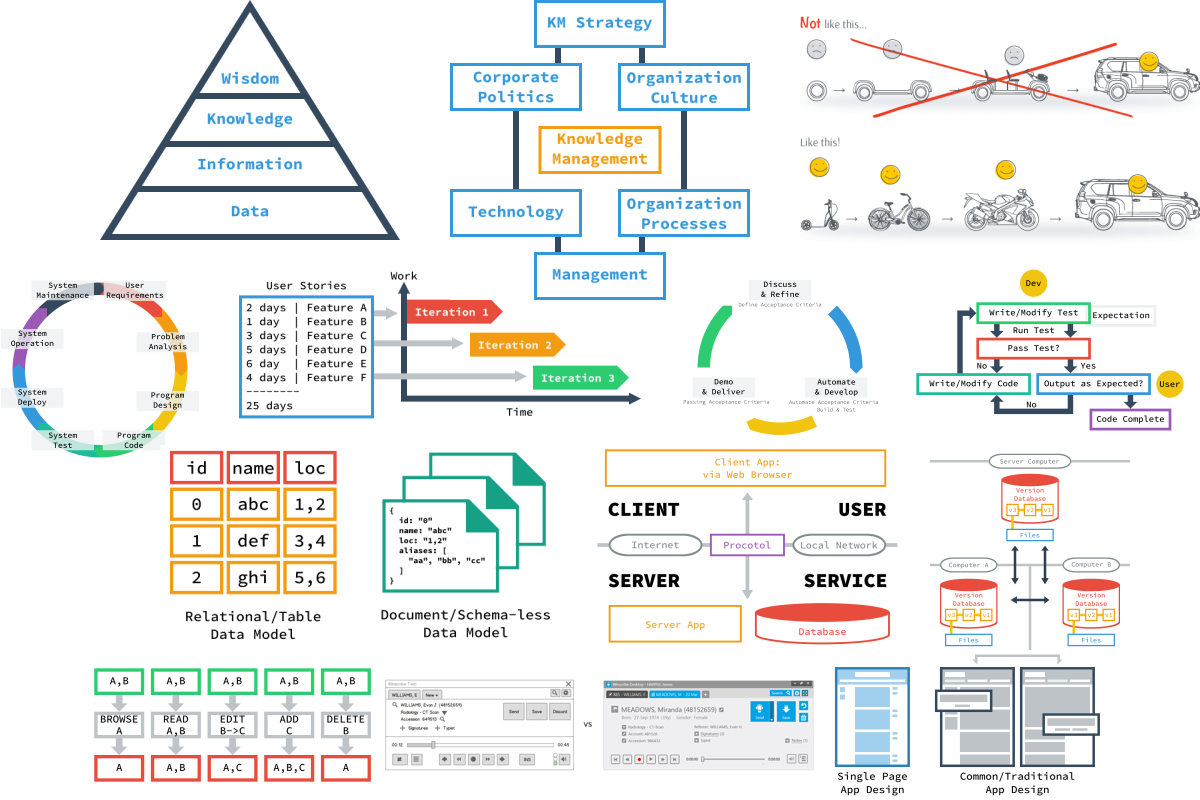
\includegraphics[width=11cm]{include/literature-fundamentals.png}
    \label{fig:literature-fundamentals}
  \end{figure}

\end{frame}

% ------------------------------------------------------------

\begin{frame}
  \frametitle{Literature Study}

  \begin{figure}[ht]
    \vspace{-25pt}
    \centering
    
\includegraphics[width=11cm]{include/literature-technologies.png}
    \label{fig:literature-technologies}
  \end{figure}

\end{frame}

% ------------------------------------------------------------

\begin{frame}[fragile]
  \frametitle{Literature Study}

  \begin{block}{Knowledge Management System}
    Data-Information-Knoweldge-Wisdom (\alert{DIKW}),\\
    Knowledge Management System (\alert{KMS}), \alert{Personal Knowledge Manager}
  \end{block}

  \begin{block}{Software Development Life Cycle}
    \alert{Agile} methodologies, Minimum Viable Product (\alert{MVP}),\\
    Acceptance Test Driven Development (\alert{ATDD})
  \end{block}

\end{frame}

% ------------------------------------------------------------

\begin{frame}[fragile]
  \frametitle{Literature Study}

  \begin{block}{Design Pattern}
    \textsc{browse, read, edit, add, delete} (\alert{BREAD}),\\
    simple interaction and interface design with mockup,\\
    and Single Page Application (\alert{SPA})
  \end{block}

  \begin{block}{Database}
    \alert{NoSQL}, document database, \alert{MongoDB}
  \end{block}

  \begin{block}{Programming}
    \alert{JavaScript}, \alert{JSON}, \alert{Node.js}, web application, \alert{framework}, full stack framework called \alert{Meteor}, source code management (\alert{SCM}) with \alert{Git}
  \end{block}

\end{frame}

% ============================================================

\section{Analysis \& Design}

% ------------------------------------------------------------

\begin{frame}
  \frametitle{Satellid}

  \begin{figure}[ht]
    \centering
    \includegraphics[width=8cm]{include/satellid-logo.png}
    \label{fig:satellid-logo}
  \end{figure}

\end{frame}

% ------------------------------------------------------------

\begin{frame}[fragile]
  \frametitle{Analysis}

    \begin{block}{Target user:}
      Person who frequently gather and need to manage their knowledge at almost everytime.
    \end{block}

    \begin{block}{User Types:}
      New user, existing user, regular person, researcher, engineer,
      developer, designer, information architect, event speaker,
      student, teacher, leader, collaborator, colleagues, recruiter, etc
    \end{block}

\end{frame}

% ------------------------------------------------------------

\begin{frame}[fragile]
  \frametitle{Analysis}

  Agile User Stories
  \begin{enumerate} \itemsep0pt
    \item As a System, I need to be run on supported platform and via a network
    \item As a System, I can have the data imported without the app opened
    \item As a User, I want to use the app via web browser
    \item As a User, I want to read knowledge that already stored
    \item As a User, I want to search a knowledge and browse the search result
    \item As a User, I want to add a new knowledge based on context
    \item As a User, I want to delete a stored knowledge
    \item As a User, I want to edit a stored knowledge
  \end{enumerate}

\end{frame}

% ------------------------------------------------------------

\begin{frame}[fragile]
  \frametitle{Design}

  \begin{block}{Contextual System}
    A data and template approach to classify the knowledge with its context and structure.
  \end{block}

\end{frame}

% ------------------------------------------------------------

\begin{frame}[fragile]
  \frametitle{Design}

  \begin{figure}[ht]
    \centering
    \includegraphics[width=9cm]{include/satellid-contextual.png}
    \caption{Contextual System}
    \label{fig:satellid-contextual}
  \end{figure}

\end{frame}

% ------------------------------------------------------------

\begin{frame}[fragile]
  \frametitle{Design}

  Functionality Flow
  \begin{enumerate} \itemsep0pt
    \item Turn on and turn off the System via terminal/CLI.
    \item Access and use the System via Web browser.
    \item Type and search in the search bar that could automatically show the search result.
    \item Browse the existing knowledge or search result in the collection of cards.
    \item Add a knowledge that will show the form box to fill.
    \item Edit a knowledge with edit mode of form box.
    \item Delete a knowledge.
  \end{enumerate}

\end{frame}

% ------------------------------------------------------------

\begin{frame}[fragile]
  \frametitle{Design}

  \begin{figure}[ht]
    \centering
    \includegraphics[height=6.5cm]{include/satellid-app-arch.png}
    \caption{Application Architecture}
    \label{fig:satellid-app-arch}
  \end{figure}

\end{frame}

% ------------------------------------------------------------

\begin{frame}[fragile]
  \frametitle{Design}

  \begin{figure}[ht]
    \centering
    \vspace{-25pt}
    \includegraphics[height=7.5cm]{include/satellid-app-ui.png}
    \caption{User Interface Mockup Design}
    \vspace{-20pt}
    \label{fig:satellid-ui}
  \end{figure}

\end{frame}

% ------------------------------------------------------------

\begin{frame}[fragile]
  \frametitle{Design}

  \begin{figure}[ht]
    \centering
    \vspace{-25pt}
    \includegraphics[width=8cm]{include/satellid-app-uix.png}
    \vspace{-20pt}
    \caption{User Interaction Design}
    \label{fig:satellid-uix}
  \end{figure}

\end{frame}

% ============================================================

\section{Implementation \& Testing}

% ------------------------------------------------------------

\begin{frame}[fragile]
  \frametitle{Implementation}

  Snippets of Server Code
  \begin{minted}[fontsize=\small]{javascript}
    if (Meteor.isServer) {
      Meteor.startup(function() {
        ...
      });
    }
  \end{minted}

  Snippets of Client Code
  \begin{minted}[fontsize=\small]{javascript}
    if (Meteor.isClient) {
      Template.add.events({
        "click button": function() {
          ...
        }
      });
    }
  \end{minted}

\end{frame}

% ------------------------------------------------------------

\begin{frame}[fragile]
  \frametitle{Implementation}

  \begin{figure}[ht]
    \centering
    %TODO-SCREEN
    \vspace{-25pt}
    \includegraphics[height=7.5cm]{include/satellid-app-result.png}
    \vspace{-10pt}
    \caption{Application Result Screenshot}
    \label{fig:satellid-app-result}
  \end{figure}

\end{frame}

% ------------------------------------------------------------

\begin{frame}[fragile]
  \frametitle{Testing}

  \begin{figure}[ht]
    \centering
    \includegraphics[height=6.5cm]{include/satellid-app-test.png}
    \caption{Testing Screenshot}
    \label{fig:satellid-app-test}
  \end{figure}

\end{frame}

% ============================================================

\section{Closing}

% ------------------------------------------------------------

\begin{frame}[fragile]
  \frametitle{Conclusion}

  \begin{enumerate}
    \item Simple and single system of managing tons of personal daily knowledge
    \item Implementation with Web technologies
    \item Flexible data schema combined with template
    \item Template based on context
  \end{enumerate}

\end{frame}

% ------------------------------------------------------------

\begin{frame}[fragile]
  \frametitle{Suggestion \& Future Work}

  There could be some inadequacy, so further and iterated improvement will remain to be done continuously

  \begin{block}{Future Feature Roadmap:}
    Account system, easy import \& export, more predefined context and field, BREAD the template, more custom configuration, multimedia support, integration with other networks, encryption, etc
  \end{block}

\end{frame}

% ============================================================

\plain{Thank You}

% ------------------------------------------------------------

\end{document}
